
A modo de introducción, comenzaremos esta sección mostrando los datos demográficos obtenidos. Mas adelante, continuaremos con un análisis mas exhaustivo de inteligibilidad y por separado se realizará otro análisis respecto a la nacionalidad atribuida a las oraciones. Por último para evaluar la hipótesis original, compondremos estos dos ejes para dilucidar su grado de validez.

\section{Datos demográficos}

Se encuestaron $109$ participantes de los cuales se obtuvieron $352$ resultados.

Del total de participantes, $49$ pertenecían al rango comprendido entre $18$ y $25$ años, $43$ estaban en el rango $26$-$35$. $17$ de los participantes eran mayores a $35$ años (fig. \ref{genero}).

\begin{figure}
\centering
\begin{subfigure}{.5\textwidth}
  \centering
	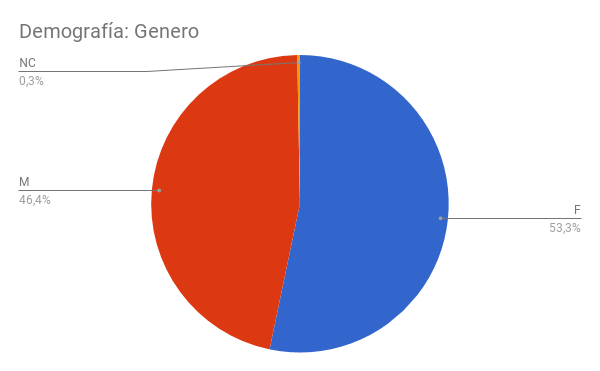
\includegraphics[width=.3\linewidth]{datosDemograficos/genero.png}
  \caption{A subfigure}
  \label{fig:sub1}
\end{subfigure}%
\begin{subfigure}{.5\textwidth}
  \centering
	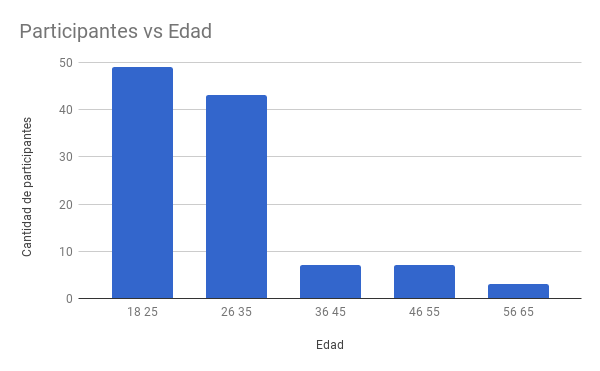
\includegraphics[width=.3\linewidth]{datosDemograficos/edad.png}
  \caption{A subfigure}
  \label{fig:sub2}
\end{subfigure}
\caption{A figure with two subfigures}
\label{fig:test}
\end{figure}

Con respecto al genero de los participantes, $187$ respuestas fueron brindadas por participantes del genero femenino mientras que $163$respuestas fueron brindadas por participante del genero masculino (fig. \ref{edad}).

En los datos referentes a la región en que cada participante pasó su infancia puede verse una predominancia de personas del Gran Buenos Aires con $45\%$, seguido por un $30\%$ que pasaron su infancia en la Capital Federal. Menos del $25\%$ pertenece al resto de las provincias Argentinas. Además, $10$ personas contestaron que se criaron fuera del país (fig. \ref{distTerritorial}).

\begin{figure}
\begin{center}
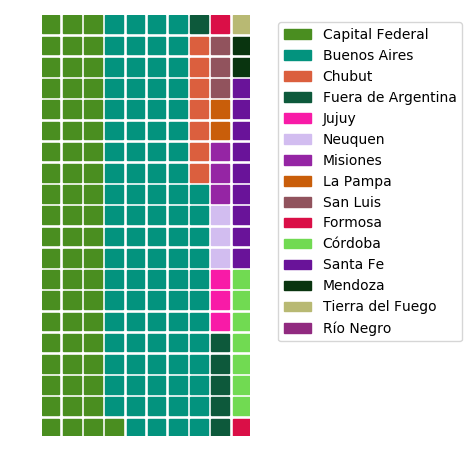
\includegraphics[scale=0.8]{datosDemograficos/infancia.png}
\end{center}
\caption{Distribución Territorial}
\label{distTerritorial}
\end{figure}

\section{Inteligibilidad}

A continuación intentaremos medir la inteligibilidad de cada una de las oraciones en base a las respuestas obtenidas por los participantes. Para ello tomaremos la oración transcripta por los participantes y mediremos cuan lejos o cerca está de la oración original. 

Para esto utilizaremos la distancia de Levenshtein, que consiste en calcular la menor cantidad posible de inserciones, remociones o reemplazos de caracteres posibles que son requeridos para transformar la oración transcripta por un participante en la oración objetivo. Así por ejemplo, para transformar \textit{cosa} en \textit{cal} se requieren $3$ transformaciones: reemplazar \textit{o} por \textit{a}, reemplazar \textit{s} por \textit{l} y remover la \textit{a} por lo que la distancia de Levinshtein entre estas dos oraciones es de $3$. Además, se considerará un remplazo cualquier acento, por lo que \textit{á} y \textit{a} tendrán distancia $1$ pero no así el reemplazo de mayúsculas y minúsculas, por lo que \textit{a} y \textit{A} tendrán distancia $0$.

En la figura \ref{resultadosGenerales} presentamos los resultados generales obtenidos sin ningún tipo de modificación.

\begin{figure}
\begin{center}$
\begin{array}{lll}
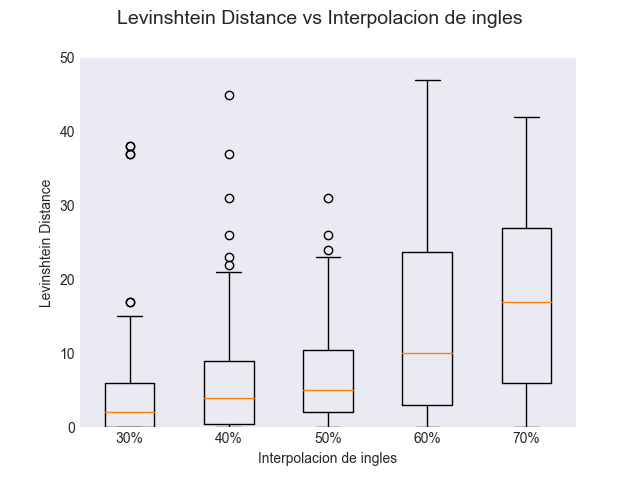
\includegraphics[width=.7\textwidth]{imagenes/plots_raw/general.png}
\end{array}$
\end{center}
\caption{Resultados Generales}
\label{resultadosGenerales}
\end{figure}

Como puede observarse hasta el $50\%$ de mezcla castellano-ingles, la distancia entre el primer y tercer cuartil menor a $10$ caracteres, siendo la media de $5$ caracteres. Pasados el $60\%$ de ingles, se observa un aumento brusco el la distancia intercuartiles, la distancia entre el primer y tercer cuartil pasa a ser cercana a $20$ caracteres, y la media $10$ caracteres en el caso de $60\%$ ingles y $15$ en el caso del $70\%$. En las proximas secciones intentaremos encontrar una explicación intuitiva a estos números.

\section{Problemas en las transcripciones y normalización}

Analizando detenidamente las transcripciones obtenidas pudimos observar algunas fallas sistemáticas que podrían generar ruido en el análisis, por ejemplo algunos de los participantes escribieron de manera diferente las secciones de la oración que no comprendieron. Por citar algunos ejemplos, muchos de ellos escribieron: ``...'', ``....'' o simplemente omitieron la palabra, mientras que una minoría escribió cosas como ``***'', ``???'', \textit{blablabla}. En los casos donde el participante no comprendió ningún segmento de la oración, es común observar expresiones como \textit{no entendí nada}, \textit{nada}, etc.

Por otra parte es común la utilización innecesaria de signos de puntuación. Estos varían desde puntos finales para expresar el final de la oración hasta expresiones de confusión tales como ``(?)''. En un caso extremo, un participante el participante transcribió \textit{``tu estrecho posavasos'', grito la fechoría}, cuando la oración original solo decía \textit{tu estrecho portavasos gritó la fechoría}.
También pueden verse omisiones de acentos y faltas ortográficas en palabras que no presentan ambigüedades, como por ejemplo: ``grunion'' en vez de ``gruñón''.

Para disminuir ruido de la muestra, se decidió realizar una limpieza de los datos donde consideramos que no era disruptiva.

Los cambios fueron:

\begin{itemize}
	\item Corregir ``ni'' por ``ñ'' en la palabra \textit{grunion}.
	\item Remoción de todos los signos de puntuación: comas, puntos, ``(?)''
	\item Reemplazo de oraciones como \textit{blabla}, \textit{no entendí} o cualquier otra expresión que indique ininteligibilidad de una palabra u oración por ``''.
	\item Corrección de acentos en palabras no ambiguas: \textit{botón}, \textit{prefirió}, \textit{recorrió}, \textit{chupetín}, \textit{riñon}, \textit{gruñón}.
\end{itemize}

Aquellas palabras que presentan ambivalencia, como : \textit{concluyó} no fueron modificadas ya que tanto \textit{concluyó/concluyo} son validas. El participante podría haber interpretado la palabra con cualquiera de las dos connotaciones cambiando el significado de la interpretación.

Esperamos que esta normalización no solamente ayude a disminuir la propagación de los resultados, sino que además, nos permitirá interpretar de manera mas intuitiva el significado la distancia de Levenshtein en cada caso.

\clearpage

\section{Datos normalizados}

Podemos observar en la figura \ref{generalNormalizado} los nuevos resultados con los datos normalizados. Para $40\%$ y $50\%$ ingles . Para $60\%$ . Para $70\%$ .

\begin{figure}
\begin{center}$
\begin{array}{lll}
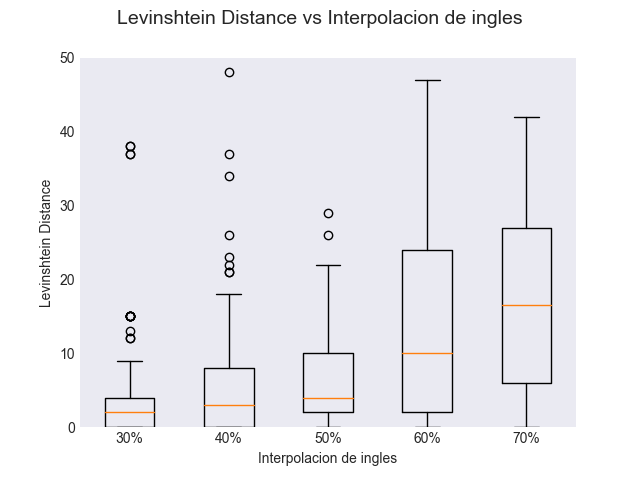
\includegraphics[width=.7\textwidth]{imagenes/plots_normalized/general.png}
\end{array}$
\end{center}
\caption{General Normalizado}
\label{generalNormalizado}
\end{figure}

Con este baseline, podemos ver que para una interpolación de ingles de $30\%$, $96$ de los $106$ participantes obtuvieron una distancia menor a los $10$ caracteres en la transcripción del texto, mientras que los $10$ restantes una distancia mayor a los 10 caracteres. Podemos ver además que la distancia entre el primer y tercer cuartil es menor a $5$ caracteres con una media cercana a $2$ 

Para la mezcla $40\%$ ingles - $60\%$ castellano, de un total de $67$ participantes, $57$ anotaron una distancia de Levinshtein menor a diez caracteres, $7$ una distancia entre $10$ y $30$ caracteres y $3$ una distancia mayor a $30$. La distancia intercuartil es de aproximadamente diez caracteres, con una media muy similar a la mezcla $30\%$ ingles.

Para la interpolación $50\%$ ingles - $50\%$ castellano, de un total de $75$ participantes, $57$ lograron transcribir el audio con una distancia menor a 10 caracteres, mientras que $14$ anotaron una distancia entre $10$ y $20$ caracteres y $4$ una distancia mayor a $20$. De manera similar que para $40\%$ la distancia intercuartil es de aproximadamente diez caracteres y la media es de $3$ caracteres.

Con esta estandarización de los datos, trataremos de darles un peso intuitivo que nos permitan sistematizar el análisis.

Por ejemplo, tomando la oración $8$ de las frases utilizadas en la experimentación: 

\begin{itemize}
	\item ``Las acongojadas cotorras sonrieron a mi círculo''
\end{itemize}

Podemos observar las siguientes transcripciones extraídas de los resultados:

\begin{itemize}
	\item Distancia 0: ``Las acongojadas cotorras sonrieron a mi círculo''
	\item Distancia 10: ``Las acontojadas culturas sonrieron en semicírculo''
	\item Distancia 20: ``Plaza sombreada con sombrero sonrieron en mi círculo''
	\item Distancia 30: ``sonrieron en mi círculo''
	\item Distancia 40: ``círculo''
	\item Distancia 48: ``''
\end{itemize}

Para todas las interpolaciones enunciadas previamente, los errores mas comunes varían desde falta de acentos en palabras como ``concluyó'' hasta faltas de inteligibilidad en palabras con cierta complejidad fonética como ``aguileña'' o ``gruñón''.

Como caso particular la oración $3$: ``este enjoyado juez comprará nuestro corchete'' podemos observar que la mayoría de los participantes cometieron errores al transcribir la palabra ``juez'' que confundieron de manera sistemática con palabras sonoramente similares como ``fue'', y ``enjoyado'' que transcribieron como ``enfollado'', ``enrollado'' y la conjugación exacta del verbo comprar.

Para los grados de interpolación $60\%$ ingles - $40\%$ castellano y $70\%$ ingles - $30\%$ castellano, podemos observar un aumento notable de la variabilidad en las respuestas. Para el primero, de las $70$ respuestas obtenidas, $40$ participantes lograron transcribir el audio con una distancia menor a diez caracteres, $6$ obtuvieron anotaron una distancia entre $10$ y $20$ caracteres, y $24$ transcribieron el audio con distancia mayor a veinte caracteres. La distancia entre el primer y tercer cuartil pasa a ser de $20$ caracteres con una media igual a $10$.

Para $70\%$ ingles - $30\%$ castellano, la diferencia es todavía mas marcada, de los $68$ resultados obtenidos, $28$ lograron transcribir el audio con un buen grado de inteligibilidad, $8$ con un grado medio y $32$ con un grado bajo o nulo de inteligibilidad. La distancia intercuartil se mantiene similar a la de mezcla $60\%$ ingles, aproximadamente $20$ caracteres pero vemos un salto en la media que ahora es de $20$ caracteres.

Consideramos que este salto en la distancia intercuartil puede deberse a dos motivos:

El primero es que existen características particulares de los participantes y sus capacidades para discernir palabras incluso cuando presentan defectos en la pronunciación del hablante. En particular, la oración $4$ (ver figura \ref{oracionCuatro}) muestra como para el mismo grado de interpolación, con características similares $2$ participantes de los $9$ que realizaron la transcripción, obtuvieron distancias $2$ y $6$ en sus transcripciones.

\begin{figure}
\begin{center}$
\begin{array}{lll}
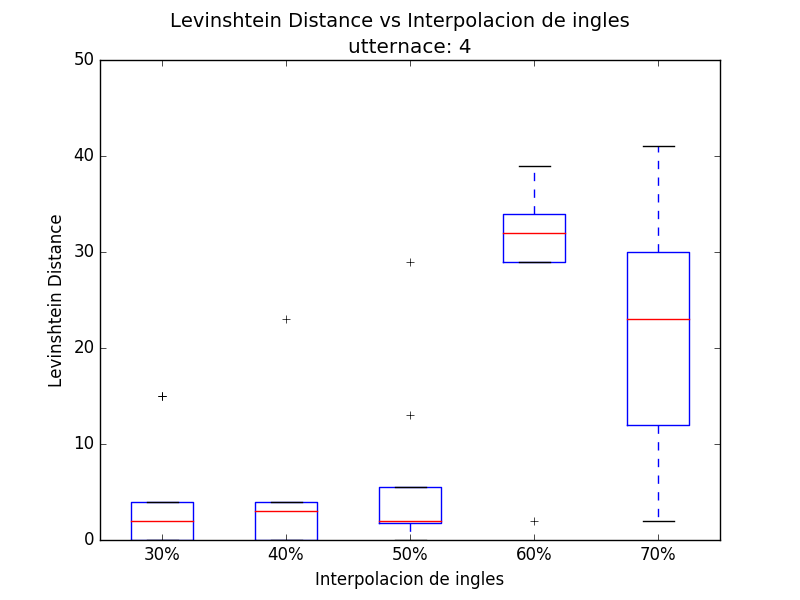
\includegraphics[width=.5\textwidth]{imagenes/plots_normalized/4.png}
\end{array}$
\end{center}
\caption{Oraciones 3 y 4 Normalizados}
\label{oracionCuatro}
\end{figure}

El segundo motivo puede deberse a que existen características particulares de las oraciones o del modelo utilizado para generar la voz que afectan la comprensión del audio: la oración $10$, donde el $6$ de los $8$ participantes obtuvieron una buena transcripción del audio, y la oración $8$, donde todos los participantes transcribieron el audio con inteligibilidad baja o nula, parecen demostrar esto. O bien la dificultad de las oraciones es variable o, lo que es todavía mas probable, llegado cierto punto en la interpolación, algunos fonemas empiezan a ``romperse'' o se alejan demasiado del fonema castellano correcto y terminan por disminuir la claridad de la voz.

\begin{figure}
\begin{center}$
\begin{array}{lll}
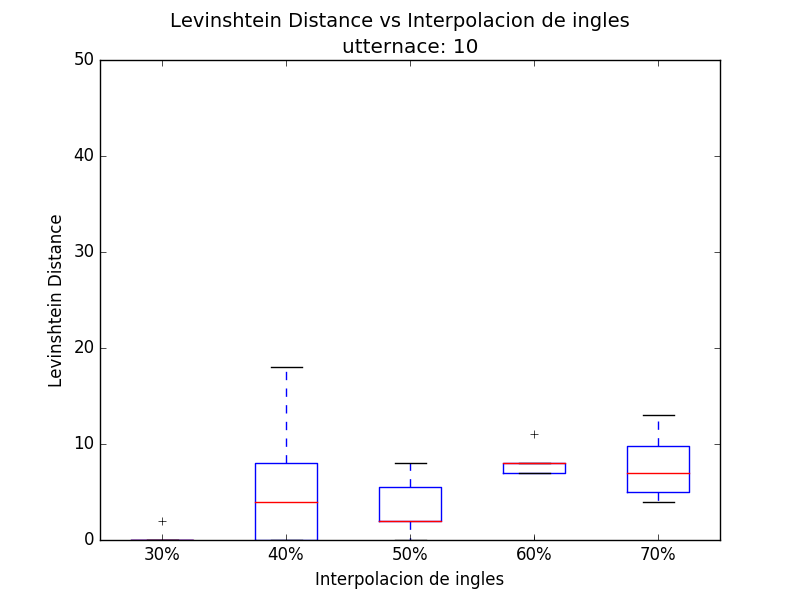
\includegraphics[width=.5\textwidth]{imagenes/plots_normalized/10.png}&
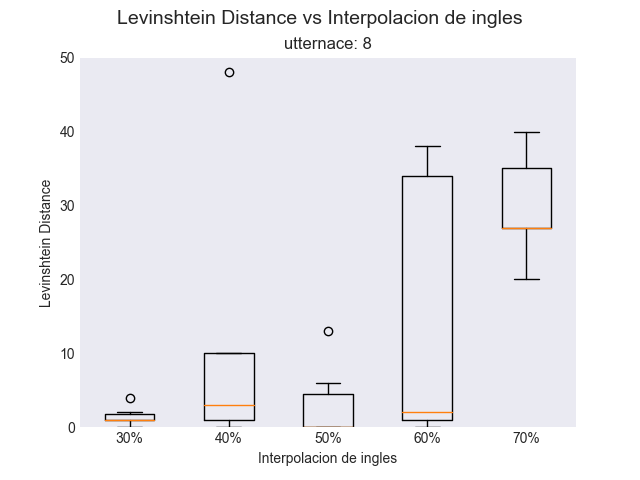
\includegraphics[width=.5\textwidth]{imagenes/plots_normalized/8.png}
\end{array}$
\end{center}
\caption{Oración 10 y 8 Normalizados}
\label{pics:blablabla}
\end{figure}

En conclusión, en esta sección pudimos demostrar que fue posible generar una voz con una distancia menor a $10$ caracteres hasta un $50\%$ de ingles y $50\%$ de castellano. Pasado el $50\%$ de ingles, la variabilidad de las respuestas se vuelve mucho mas grande pudiendo haber participantes que anotan una buena distancia de Levinshtein ($10$ caracteres o menos) hasta algunos que no logran comprender ni siquiera segmentos aislados del mismo (mas de $30$ caracteres).

% \begin{figure}
% \begin{center}$
% \begin{array}{lll}
% 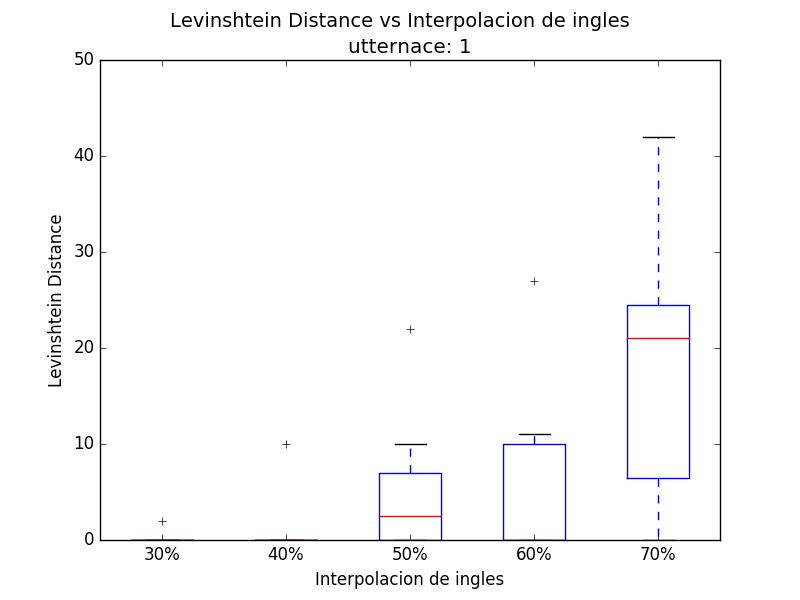
\includegraphics[width=.5\textwidth]{imagenes/plots_normalized/1.png}&
% 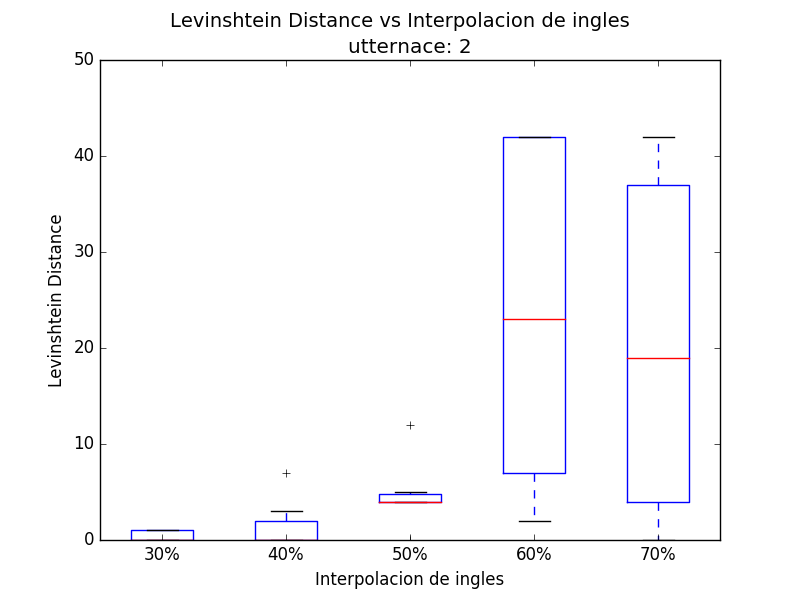
\includegraphics[width=.5\textwidth]{imagenes/plots_normalized/2.png}
% \end{array}$
% \end{center}
% \caption{Utternace 1 y 2 Normalizados}
% \label{pics:blablabla}
% \end{figure}

% \begin{figure}
% \begin{center}$
% \begin{array}{lll}
% 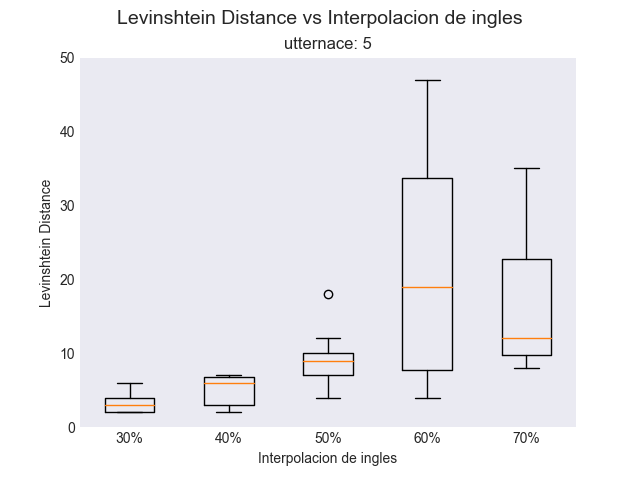
\includegraphics[width=.5\textwidth]{imagenes/plots_normalized/5.png}&
% 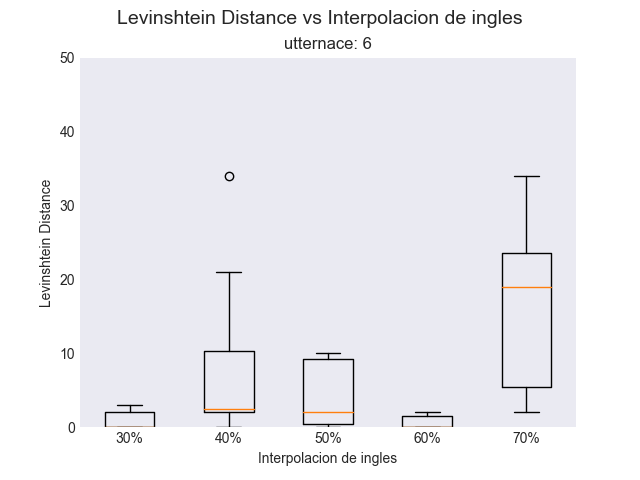
\includegraphics[width=.5\textwidth]{imagenes/plots_normalized/6.png}
% \end{array}$
% \end{center}
% \caption{Utternace 5 y 6 Normalizados}
% \label{pics:blablabla}
% \end{figure}

% \begin{figure}
% \begin{center}$
% \begin{array}{lll}
% 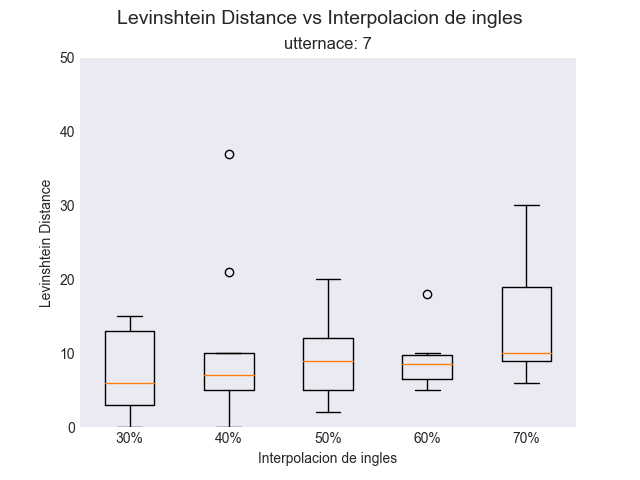
\includegraphics[width=.5\textwidth]{imagenes/plots_normalized/7.png}&
% 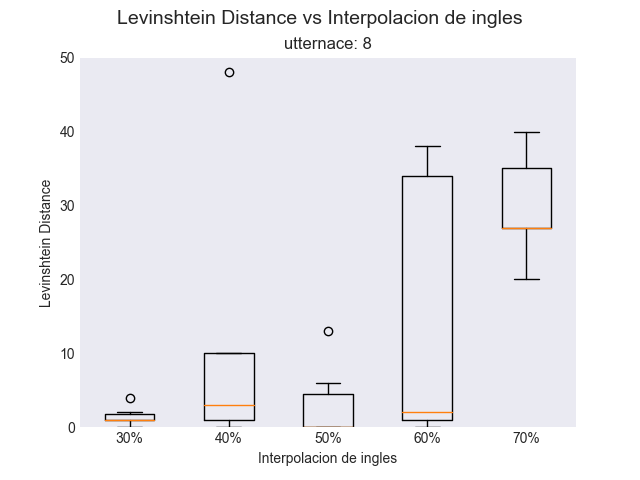
\includegraphics[width=.5\textwidth]{imagenes/plots_normalized/8.png}
% \end{array}$
% \end{center}
% \caption{Utternace 7 y 8 Normalizados}
% \label{pics:blablabla}
% \end{figure}


%Agregar:
% python levinshteinFor.py 0
% Alta int: 96
% Media int: 10
% Baja int: 0
% nula: 4
% python levinshteinFor.py 1
% Alta int: 57
% Media int: 2
% Baja int: 5
% nula: 3
% porque nula? ver esto: parecen ser outliers
% python levinshteinFor.py 2
% Alta int: 57
% Media int: 14
% Baja int: 4
% nula: 0
% python levinshteinFor.py 3
% Alta int: 40
% Media int: 6
% Baja int: 11
% nula: 13
% python levinshteinFor.py 4
% Alta int: 28
% Media int: 8
% Baja int: 20
% nula: 12


\clearpage
\section{Análisis del Órigen Percibido}

En esta sección analizaremos los resultados de las nacionalidades que los participantes de la encuesta atribuyeron a la voz.

Dado que en esta instancia se le permitió a los participantes ingresar texto libre las respuestas resultaron bastante heterogéneas. Los participantes tomaron la consigna de manera diferente, pudiendo encontrarse respuestas que no pueden ser atribuidas a una nacionalidad. Como ejemplo de algunas respuestas pueden encontrarse cosas como: Latino, Anglo, Robot, España (sur).

Consideramos que las respuestas de la índole ``robot'', ``es una voz artificial'', no son validas ya que no aportan información para esta investigación.

Por esta razón, en esta instancia decidimos agrupar las respuestas en cuatro grupos:

\begin{itemize}
	\item Hispanohablante: ``Latino'', ``Argentino'', ``Español'', ``Uruguayo'', ``Centroamericano'', ``Boliviano'', `` Mexicano'',``Colombiano''.
	\item Angloparlante: ``Estadounidense'', ``Ingles'', ``Irlandés'', ``Canadiense'', ``Anglo''.
	\item No sabe/No contesta: ``Robot'', ``no se''.
	\item Otro: ``Ruso'', ``Brasiltiño''.
\end{itemize}

Con estas agrupaciones, en la figura \ref{analGeneral} presentamos las nacionalidades atribuidas a la voz generada para cada punto de la interpolación.

\begin{figure}
\begin{center}$
\begin{array}{lll}
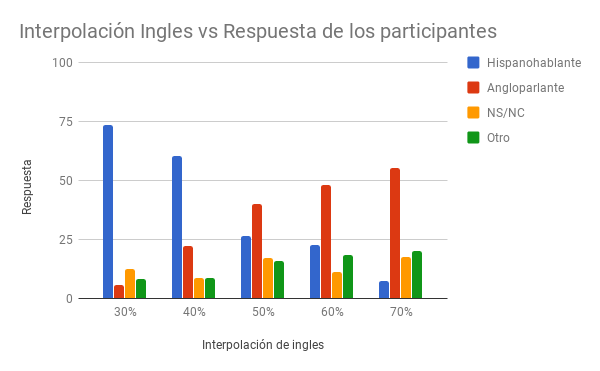
\includegraphics[width=.5\textwidth]{imagenes/nacionalidades/general.png}
\end{array}$
\end{center}
\caption{Análisis General}
\label{analGeneral}
\end{figure}

De estos resultados podemos observar que con $30\%$ de interpolación de ingles, los participantes coinciden en que la voz puede atribuirse a una persona de habla nativa española.

Con $50\%$ y $60\%$ de ingles los resultados son similares. obtenemos que aproximadamente en el $50\%$ de las oraciones, mas de la mitad de los participantes consideraron que la voz pertenecía a un anglosajón hablando castellano. Para estos grados de interpolación también podemos observar que en un $80\%$ de las oraciones al menos un $20\%$ de los participantes atribuyen la nacionalidad del hablante a un no nativo no anglosajón hablando castellano.


Con $70\%$ de interpolación, en el $80\%$ de las oraciones se puede apreciar que al menos $50\%$ de los participantes dijo que el hablante era de origen anglosajón. Mas aún, en el $40\%$ de las oraciones el $75\%$ de los participantes coincidió que la voz era de angloparlante. También podemos ver que para este grado de interpolación en el $70\%$ de las oraciones ningún participante considera que la voz sea de habla hispana. En el $30\%$ restante, $25\%$ de los participantes o menos consideran que la voz pertenezca a un hispanohablante.

%grafico general mostrando como crece el grado de ingles?

%conclucion mas general: aunque en muchos casos los participantes atribuyeron a la voz como un extrangero no anglosajon, tambien tener en cuenta que se esta intentando identificar la nacionalidad de un hablante con tan solo con una oración como referencia.

Observando las oraciones una por una, podemos observar algunas particularidades. para $40\%$ ingles, puede verse que no hay una votación homogénea. Por ejemplo en la figura \ref{tresNueve} en la oración $3$ el $80\%$ de los participantes coincide que la voz pertenece a un hablante de habla hispana, mientras que en la oración $9$ el $60.00\%$ de los participantes considera que la voz pertenece a un hablante de habla anglosajona.

\begin{figure}
\begin{center}$
\begin{array}{lll}
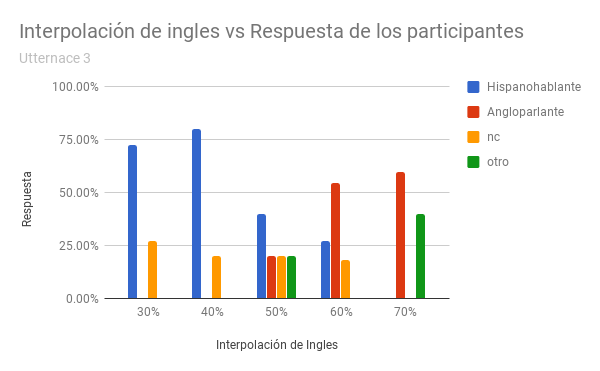
\includegraphics[width=.5\textwidth]{imagenes/nacionalidades/3.png}&
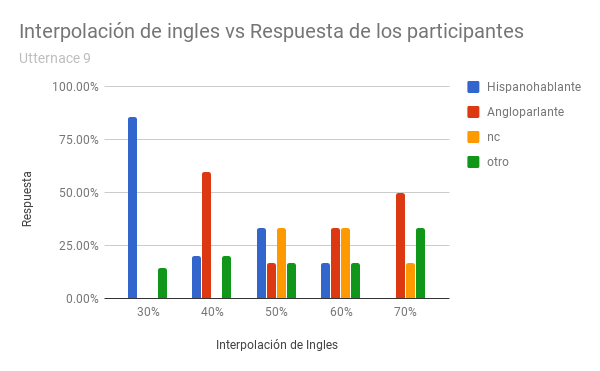
\includegraphics[width=.5\textwidth]{imagenes/nacionalidades/9.png}
\end{array}$
\end{center}
\caption{Oración 3 y 9}
\label{tresNueve}
\end{figure}

Esta gran disparidad de resultados entre distintas oraciones se puede atribuir a las características particulares de cada oración. En particular la oración $9$: ``Ese gruñón perro prometió a esos cuñados'' contiene una /\textipa{r}/ que resulta muy notoria al pronunciarse con una intensidad menor a la esperada (mas similar a una /\textipa{R}/) y es atribuida, en general, a un hablante extranjero.
%perro vibrante múltiple alveolar sonora

Bajo esta suposición observamos que las otras oraciones que presentan este fonema:

\begin{itemize}
\item Oración $1$: ``Mi montaña aguileña recorrió la esquina'' 
\item Oración $6$: ``Su profundo riñón apoyó a Julio''
\item Oración $7$: ``El frío churrasco oyó lo de Polonia''
\item Oración $8$: ``Las acongojadas cotorras sonrieron a mi círculo''
\end{itemize}

\begin{figure}
\begin{center}$
\begin{array}{lll}
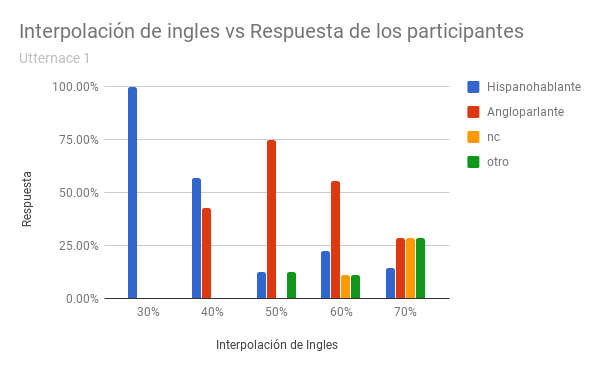
\includegraphics[width=.5\textwidth]{imagenes/nacionalidades/1.png}&
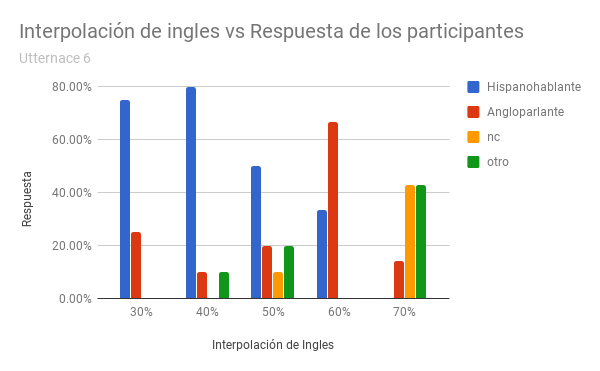
\includegraphics[width=.5\textwidth]{imagenes/nacionalidades/6.png}
\end{array}$
\end{center}
\caption{Oración 1 y 6}
\label{pics:blablabla}
\end{figure}

También presentan un mayor porcentaje de atribuciones a nacionalidad anglosajona.

\begin{figure}
\begin{center}$
\begin{array}{lll}
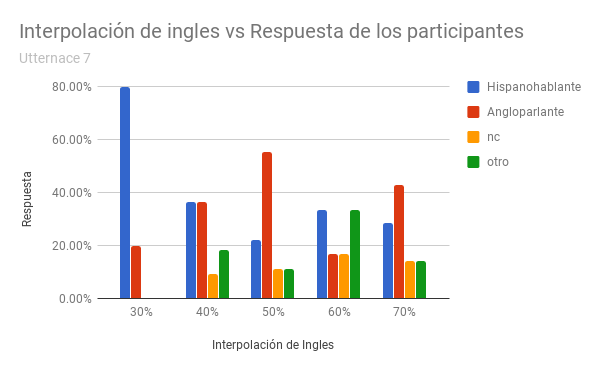
\includegraphics[width=.5\textwidth]{imagenes/nacionalidades/7.png}&
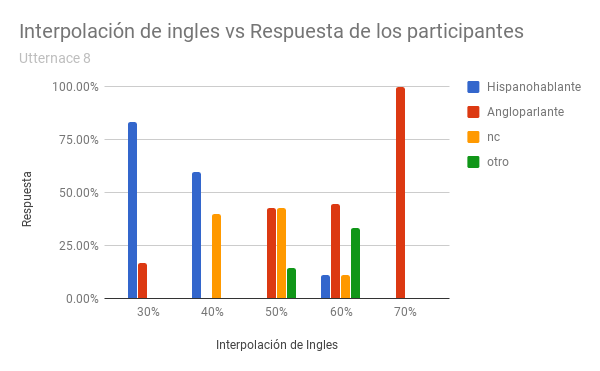
\includegraphics[width=.5\textwidth]{imagenes/nacionalidades/8.png}
\end{array}$
\end{center}
\caption{Oración 7 y 8}
\label{pics:blablabla}
\end{figure}

Hasta ahora analizamos los dos ejes de nuestra hipótesis por separado (por un lado, inteligibilidad, por otro, nacionalidad atribuida a la voz). En el ultimo apartado de la investigación buscaremos sacar conclusiones al componer ambos ejes en un mismo análisis.

\section{Resultados Generales de la experimentación}

Por ultimo visualizamos mostraremos la distancia de Levenshtein superpuesto con con la probabilidad de un participante de reconocer la voz como un hablante anglosajón.


\begin{figure}
\begin{center}$
\begin{array}{lll}
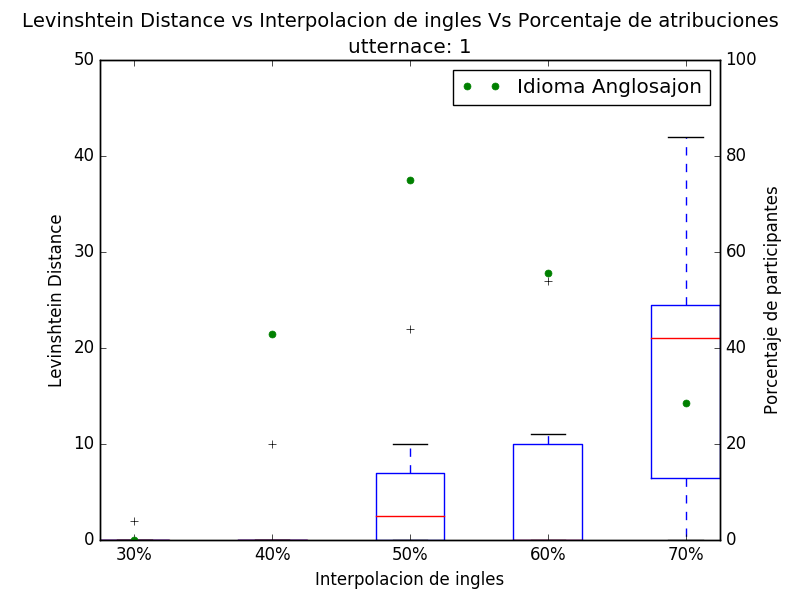
\includegraphics[width=.5\textwidth]{imagenes/nacVsPlot/1.png}&
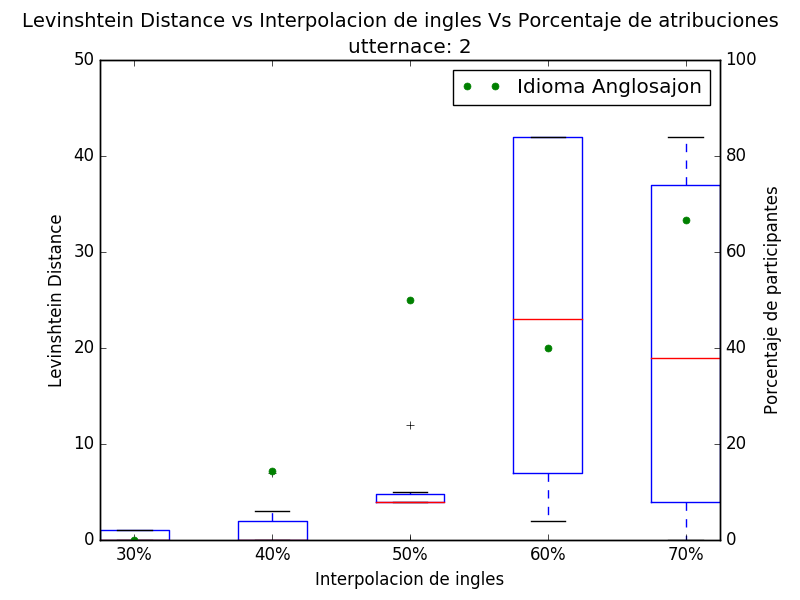
\includegraphics[width=.5\textwidth]{imagenes/nacVsPlot/2.png}
\end{array}$
\end{center}
\caption{Oración 1 y 2}
\label{pics:blablabla}
\end{figure}


Volviendo a la hipótesis original, podemos ver que esta técnica permite generar una voz que pueda ser identificada como un extranjero hablando ingles, con un grado de efectividad que varía desde el $60\%$ hasta el $100\%$ dependiendo de la oración elegido y el grado de interpolación.


\begin{figure}
\begin{center}$
\begin{array}{lll}
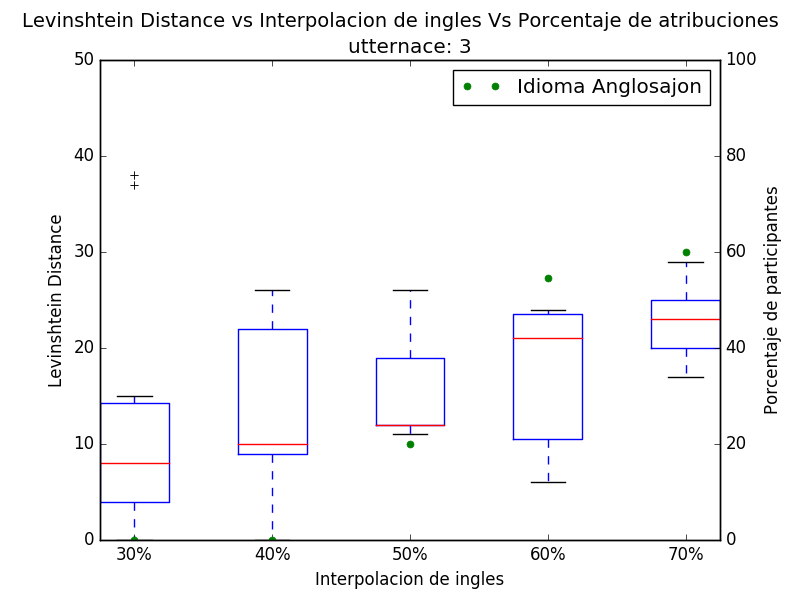
\includegraphics[width=.5\textwidth]{imagenes/nacVsPlot/3.png}&
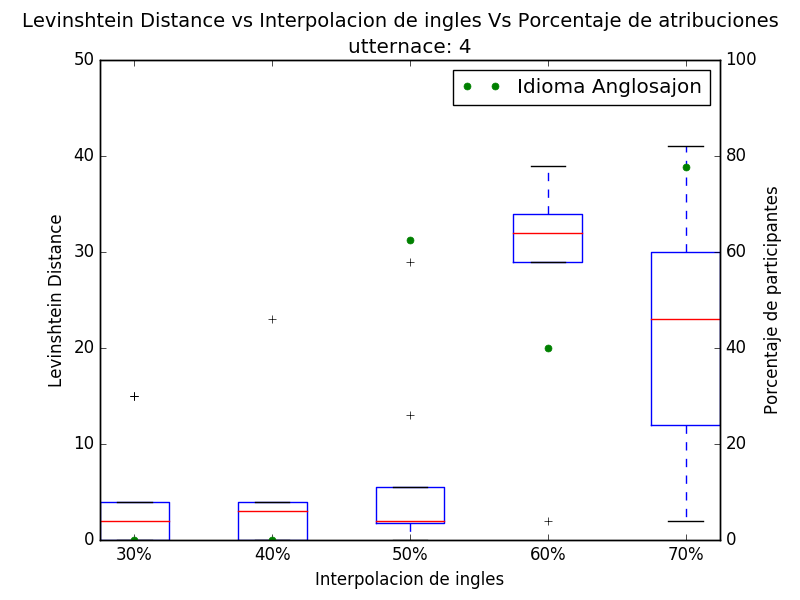
\includegraphics[width=.5\textwidth]{imagenes/nacVsPlot/4.png}
\end{array}$
\end{center}
\caption{Oración 3 y 4}
\label{pics:blablabla}
\end{figure}


También es interesante observar casos como el que se presenta comparando el oración $10$ y la oración $8$, ambos con $70\%$ de mezcla de ingles, que en cuanto a inteligibilidad se encuentran en extremos opuestos, muestran que aproximadamente un $80\%$ y un $100\%$ de participantes identificaron como nativo anglosajón. Esto nos da a pensar que la inteligibilidad de una oración y su probabilidad de ser identificado como un hablante ingles son variables independientes y que este ultimo factor este mas ligado a otros factores como la sonoridad de ciertos fonemas o la prosodia general de la voz. 


Este no es un caso aislado, véase que lo mismo sucede con la oración $4$ y $6$ con $60\%$ de mezcla de ingles, si bien las inteligibilidades están en extremos opuestos, sus probabilidades de ser identificados como hablantes extranjeros difieren en menos del $20\%$.

\begin{figure}
\begin{center}$
\begin{array}{lll}
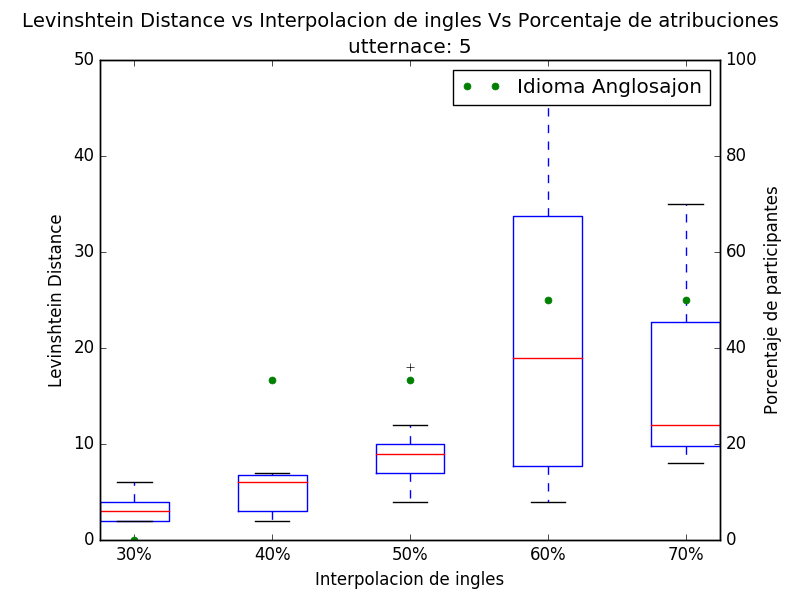
\includegraphics[width=.5\textwidth]{imagenes/nacVsPlot/5.png}&
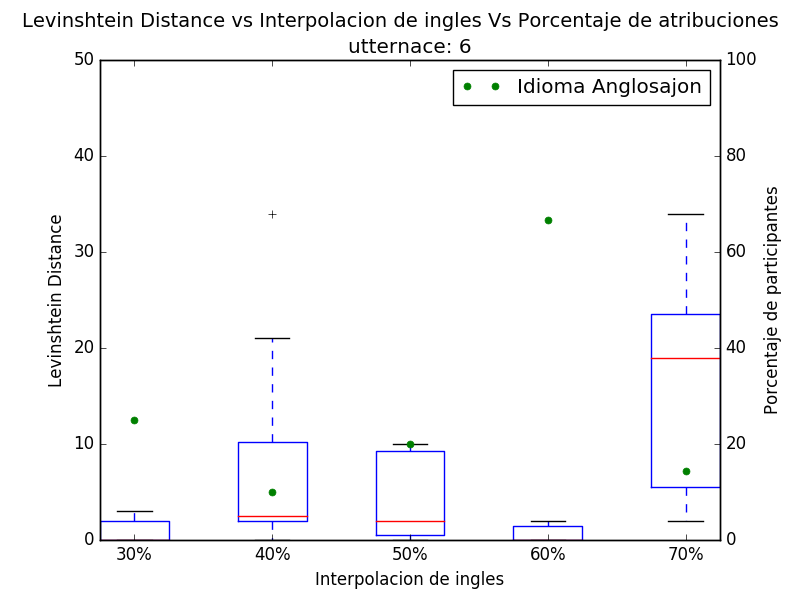
\includegraphics[width=.5\textwidth]{imagenes/nacVsPlot/6.png}
\end{array}$
\end{center}
\caption{Oración 5 y 6}
\label{pics:blablabla}
\end{figure}

\begin{figure}
\begin{center}$
\begin{array}{lll}
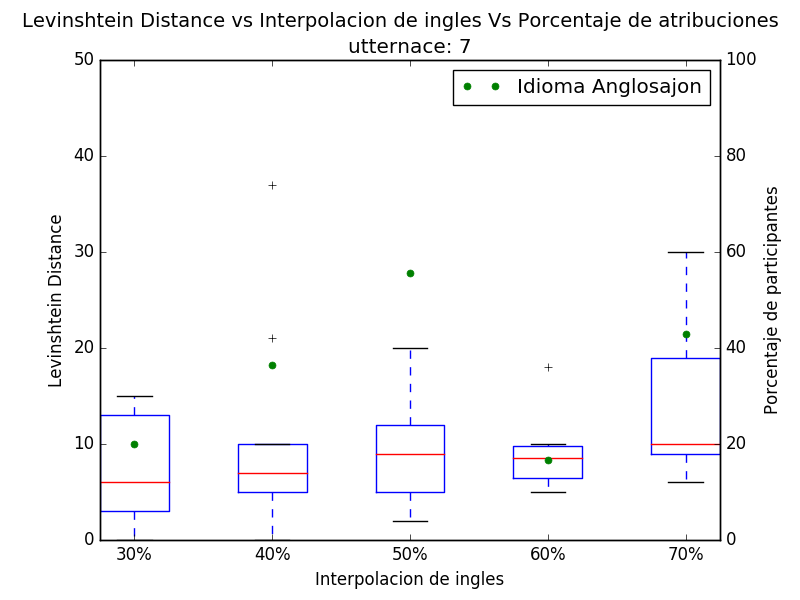
\includegraphics[width=.5\textwidth]{imagenes/nacVsPlot/7.png}&
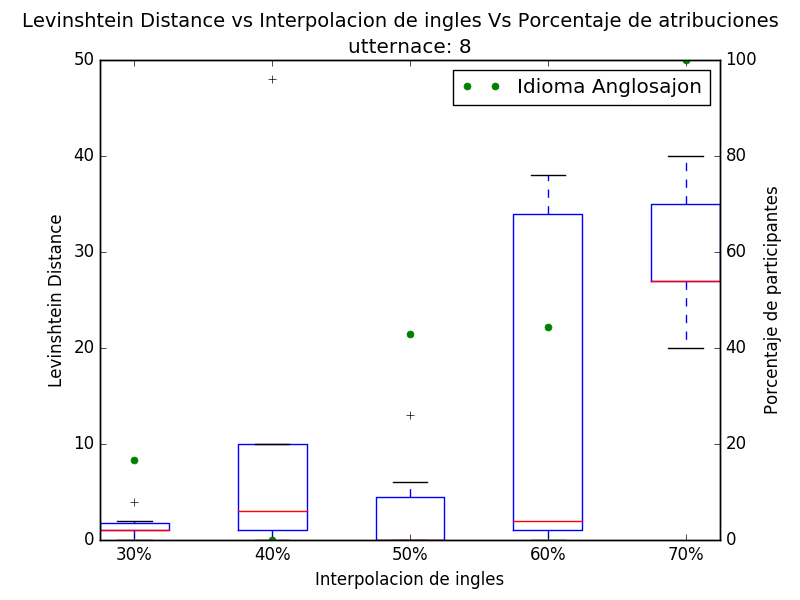
\includegraphics[width=.5\textwidth]{imagenes/nacVsPlot/8.png}
\end{array}$
\end{center}
\caption{Oración 7 y 8}
\label{pics:blablabla}
\end{figure}

\begin{figure}
\begin{center}$
\begin{array}{lll}
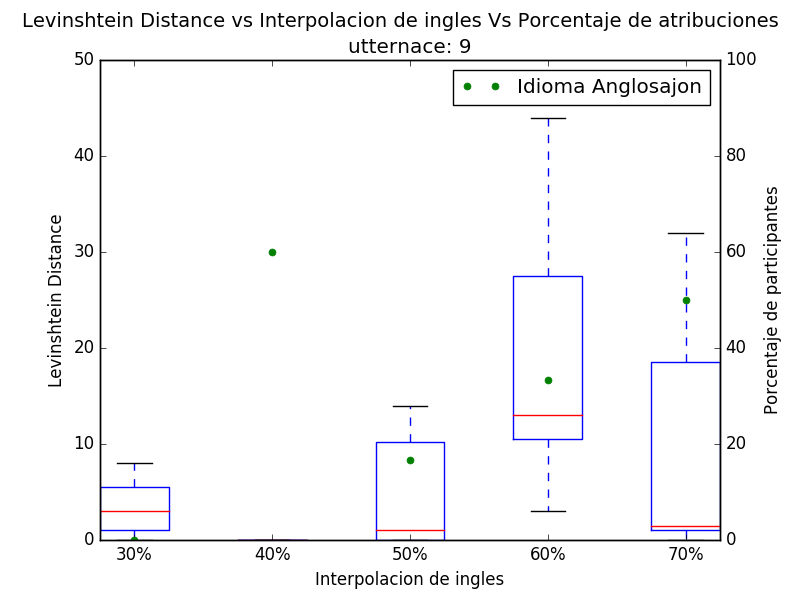
\includegraphics[width=.5\textwidth]{imagenes/nacVsPlot/9.png}&
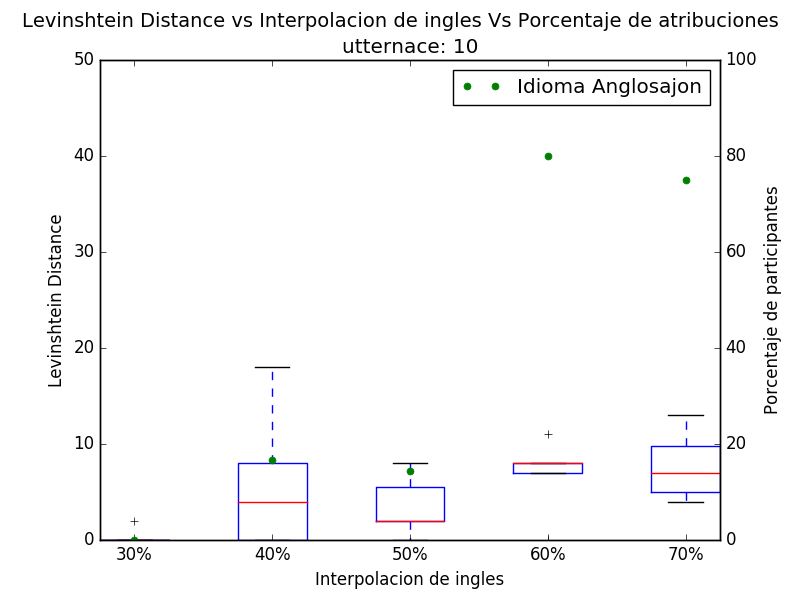
\includegraphics[width=.5\textwidth]{imagenes/nacVsPlot/10.png}
\end{array}$
\end{center}
\caption{Oración 9 y 10}
\label{pics:blablabla}
\end{figure}

